% GENERATED by harness/make_result_figures.py -- do not edit; re-run it.
% from data/exploratory_bankA_ol.json (content sha256 e0599e8fb28e9e12...)
% from data/exploratory_bankBS_ol.json (content sha256 420730f7daea008f...)
% basis: items with answer forms only (by_form_coverage.with_forms); Bank A: 13 of 14 items, 468 replies per condition; Bank B: 9 of 27 items, 324 replies per condition.
% given = leak_adj >= 0.25 (results.exceeds_threshold), all four conditions; stated = checker.check_explicit on the delivered reply, P0 and P1.
% error bars: 95% item-cluster percentile bootstrap, B=10000, seed 20261103 (items resampled); n_clusters 13 (Bank A), 9 (Bank B).
% flagged = stated in the artefact (the answer check's verdict). At P2 and P3 it is 0 by construction (the delivered text passed the same detector, or is the blocked message);
%   it is drawn as an open marker at 0 with no error bar, only where stated.<regime>.by_construction is set.
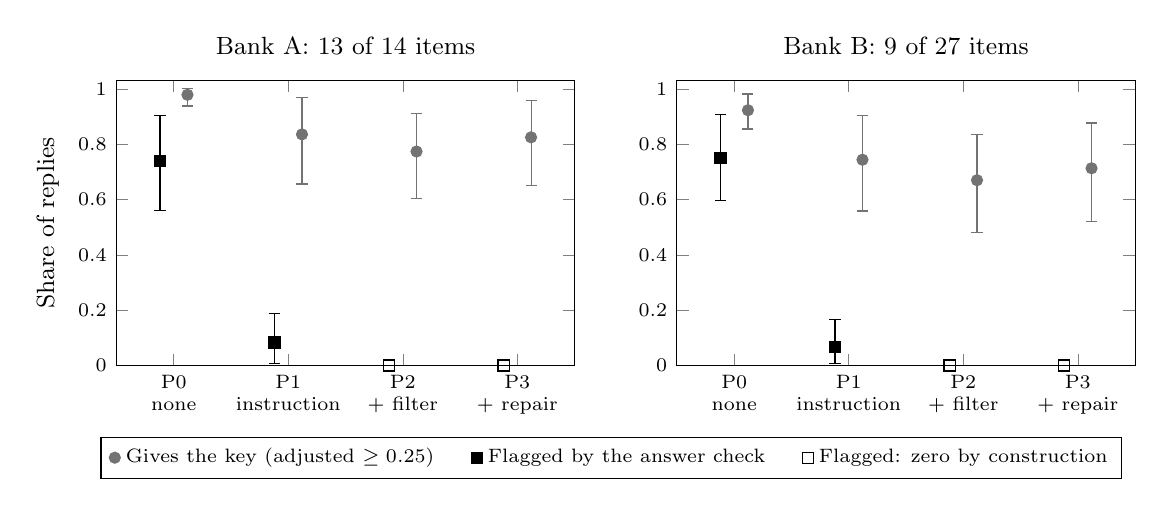
\begin{tikzpicture}
\begin{axis}[width=7.4cm,
  height=5.2cm,
  ymin=0,
  ymax=1,
  ytick={0,0.2,0.4,0.6,0.8,1},
  enlarge y limits={upper,value=0.03},
  xmin=-0.5,
  xmax=3.5,
  xtick={0,1,2,3},
  xticklabels={{P0\\none},{P1\\instruction},{P2\\+ filter},{P3\\+ repair}},
  xticklabel style={align=center},
  tick label style={font=\scriptsize},
  label style={font=\small},
  title style={font=\small},
  title={Bank A: 13 of 14 items},
  name=left,
  ylabel={Share of replies},
  legend columns=3,
  legend style={font=\scriptsize, at={(1.08,-0.25)}, anchor=north, cells={anchor=west}, /tikz/every even column/.append style={column sep=0.4cm}}]
% series: given
\addplot[only marks, mark=*, color=black!55, mark options={fill=black!55}, error bars/.cd, y dir=both, y explicit] coordinates {
  (0.12,0.9786) += (0,0.0214) -= (0,0.0406)
  (1.12,0.8355) += (0,0.1346) -= (0,0.1795)
  (2.12,0.7735) += (0,0.1389) -= (0,0.1688)
  (3.12,0.8248) += (0,0.1325) -= (0,0.1752)
};
\addlegendentry{Gives the key (adjusted $\geq 0.25$)}
% series: flagged
\addplot[only marks, mark=square*, color=black, mark options={fill=black}, error bars/.cd, y dir=both, y explicit] coordinates {
  (-0.12,0.7393) += (0,0.1645) -= (0,0.1795)
  (0.88,0.0833) += (0,0.1047) -= (0,0.0769)
};
\addlegendentry{Flagged by the answer check}
% series: flagged, zero by construction
\addplot[only marks, mark=square, color=black, mark options={fill=white}] coordinates {
  (1.88,0.0000)
  (2.88,0.0000)
};
\addlegendentry{Flagged: zero by construction}
\end{axis}
\begin{axis}[width=7.4cm,
  height=5.2cm,
  ymin=0,
  ymax=1,
  ytick={0,0.2,0.4,0.6,0.8,1},
  enlarge y limits={upper,value=0.03},
  xmin=-0.5,
  xmax=3.5,
  xtick={0,1,2,3},
  xticklabels={{P0\\none},{P1\\instruction},{P2\\+ filter},{P3\\+ repair}},
  xticklabel style={align=center},
  tick label style={font=\scriptsize},
  label style={font=\small},
  title style={font=\small},
  title={Bank B: 9 of 27 items},
  at={(left.south east)},
  anchor=south west,
  xshift=1.3cm]
% series: given
\addplot[only marks, mark=*, color=black!55, mark options={fill=black!55}, error bars/.cd, y dir=both, y explicit] coordinates {
  (0.12,0.9228) += (0,0.0587) -= (0,0.0679)
  (1.12,0.7438) += (0,0.1605) -= (0,0.1852)
  (2.12,0.6698) += (0,0.1666) -= (0,0.1883)
  (3.12,0.7130) += (0,0.1636) -= (0,0.1914)
};
% series: flagged
\addplot[only marks, mark=square*, color=black, mark options={fill=black}, error bars/.cd, y dir=both, y explicit] coordinates {
  (-0.12,0.7500) += (0,0.1574) -= (0,0.1543)
  (0.88,0.0679) += (0,0.0988) -= (0,0.0617)
};
% series: flagged, zero by construction
\addplot[only marks, mark=square, color=black, mark options={fill=white}] coordinates {
  (1.88,0.0000)
  (2.88,0.0000)
};
\end{axis}
\end{tikzpicture}
